\chapter{Parallel Algorithms: Parallel DFS}
\label{ch:parallel-algorithms}

\section*{Learning Outcomes}
\addcontentsline{toc}{section}{Learning Outcomes}

\begin{enumerate}
    \item Explain why a strict depth-first search tree is difficult to construct in parallel.
    \item Distinguish a parallel depth-biased work-pool traversal from a true DFS traversal.
    \item Describe the divide-and-conquer strategy for constructing a DFS tree using a spine path and hanging components.
    \item Use parallel spanning-tree construction, Boruvka rounds, and parallel union--find as building blocks for graph algorithms.
    \item Explain pointer jumping as a method for compressing parent pointers and identifying connected components.
    \item Construct an Euler tour representation of a tree and reduce depth/path computation to parallel list ranking.
    \item Attach off-spine connected components to the correct spine vertices using a deterministic rule.
    \item Merge independently computed DFS subtrees into a global DFS tree using subtree sizes and parallel prefix sums.
    \item Classify non-tree edges in a merged DFS tree using DFS number intervals.
    \item Reason about the gap between parallel graph traversal and a verified DFS tree.
\end{enumerate}

\section*{Recap from Previous Lecture}
\addcontentsline{toc}{section}{Recap from Previous Lecture}

\begin{itemize}
    \item Parallel algorithms must be analyzed using both \emph{work} (total operations) and \emph{span} or \emph{critical path} (longest dependence chain).
    \item Good parallel algorithms usually expose independent subproblems, avoid centralized bottlenecks, and replace serial scans with reductions or prefix sums.
    \item Graph algorithms are especially subtle because local decisions may impose global structural constraints.
    \item Synchronization primitives such as locks and atomics can make shared-state graph traversal correct, but they do not automatically preserve a desired traversal order.
    \item Prefix sums, reductions, and pointer jumping are recurring tools for turning global-looking graph operations into parallel primitives.
\end{itemize}

\section{The Problem: Why Parallel DFS Is Hard}
\label{sec:parallel-dfs-hard}

Depth-first search (DFS)\index{DFS}\index{depth-first search} is one of the cleanest serial graph algorithms:
start at a root, recursively visit one unvisited neighbour, continue down that path as far as possible, and backtrack only when the current branch is exhausted.
This description hides a strong sequential dependency.
At any moment, the next recursive call depends on the entire history of earlier choices.

\begin{ppdefn}
\ \ppterm{A DFS tree}\index{DFS tree} is the tree of first-discovery edges produced by a depth-first traversal.
For an undirected graph, every non-tree edge in a valid DFS tree connects a vertex to one of its ancestors or descendants in that tree.
This ancestor--descendant property is the structural signature that separates DFS from an arbitrary graph traversal.
\end{ppdefn}

The difficulty is not merely that DFS uses a stack.
A stack can be shared between processors.
The difficulty is that a \emph{specific DFS order} is a serial object.
If the serial rule says ``always explore the smallest unvisited neighbour first,'' then the algorithm must know whether the smallest neighbour's entire recursive subtree has finished before it is allowed to explore the next neighbour.
That decision creates a long dependence chain.

\paragraph{Intuition: Why DFS creates a dependency chain.}
A useful way to understand this dependence is to think in terms of \emph{unfinished work}. 
When DFS explores a neighbour \(v\), it is not enough to simply visit \(v\); the algorithm must completely explore the entire subtree rooted at \(v\) before returning to consider another neighbour. 
This means that the decision to explore the next neighbour is blocked until all recursive calls below the current one are finished. 
In parallel terms, this creates a strict \emph{serialization constraint}: even if multiple processors are available, they cannot safely proceed to other branches without violating DFS ordering. 
Thus, the dependency is not just about visiting nodes, but about enforcing a global completion order over recursive subtrees.

\begin{pppitfall}
\ Starting many recursive calls from the same vertex at the same time does not produce a DFS.
If a processor explores neighbour \(B\) while another explores neighbour \(C\), the resulting discovery pattern may be a useful parallel traversal, but it is not the same as depth-first exploration from \(B\) followed by backtracking to \(C\).
\end{pppitfall}

\subsection{Three Levels of Ambition}

It is useful to separate three goals:

\begin{enumerate}
    \item \textbf{Parallel search:} find reachable vertices quickly, without requiring a valid DFS tree.
    \item \textbf{Some valid DFS tree:} construct any tree satisfying the DFS ancestor--descendant property.
    \item \textbf{A specific DFS order:} reproduce a particular serial DFS order, such as smallest-neighbour-first DFS.
\end{enumerate}

The first goal is achievable with simple shared work pools.
The second is much harder and requires structural reasoning about the graph.
The third is harder still because it asks a parallel computation to reproduce a serial tie-breaking history.

\begin{ppkey}
\ The lecture focuses on the conceptual path from a simple parallel traversal to a divide-and-conquer construction of a DFS tree.
The main lesson is not that DFS becomes easy; it is that valid DFS structure must be engineered deliberately.
\end{ppkey}

\section{Work-Pool Parallel Search}
\label{sec:work-pool-search}
\index{work pool}

A natural first attempt is to keep a shared container of frontier vertices.
Many processors repeatedly remove a vertex, inspect its adjacency list, claim unvisited neighbours, and insert newly claimed vertices back into the container.
If the container is a stack, the search is \emph{depth-biased}; if it is a queue, it is breadth-biased.

\begin{figure}[h]
    \centering
    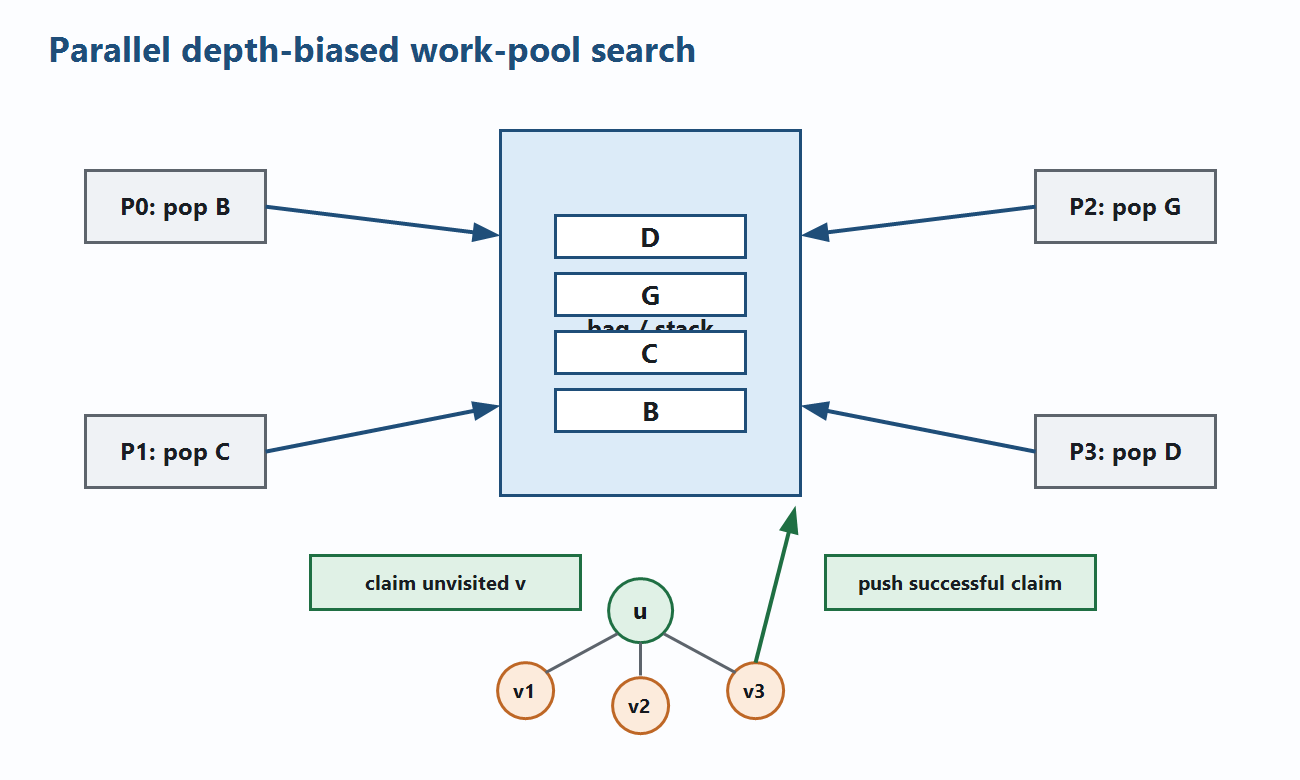
\includegraphics[width=0.92\textwidth]{media/lec26_work_pool_search.png}
    \caption{A depth-biased work pool. Processors pop frontier vertices, claim unvisited neighbours, and push successful claims back into the shared bag.}
    \label{fig:lec26-work-pool}
\end{figure}

\begin{ppprogram}{Parallel depth-biased work-pool search}{prog:work-pool-search}
\begin{lstlisting}[language=C]
parallel_work_pool_search(Graph G, Vertex r):
    for each vertex v in parallel:
        visited[v] = false
        parent[v] = NIL

    visited[r] = true
    push(pool, r)

    parallel while pool is not empty:
        u = pop(pool)
        for each neighbour v of u:
            if atomic_compare_and_swap(&visited[v], false, true):
                parent[v] = u
                push(pool, v)
\end{lstlisting}
\end{ppprogram}

The atomic compare-and-swap is essential.
Two processors may see the same unvisited neighbour \(v\) from different endpoints.
Only one processor should win the right to mark \(v\), set its parent, and push it into the pool.
Without that atomic claim, the algorithm can assign multiple parents to the same vertex.

\begin{ppdefn}
\ \ppterm{Parallel depth-biased search}\index{parallel depth-biased search} is a work-pool traversal that uses a stack-like or bag-like frontier to encourage deep exploration.
It may be effective as a reachability algorithm, but it is not guaranteed to output a strict DFS tree.
\end{ppdefn}

\begin{pppitfall}
\ The word \emph{stack} is not magic.
A shared stack gives a last-in-first-out flavour, but concurrent pushes and pops interleave nondeterministically.
The resulting parent tree depends on timing and may violate the DFS ancestor--descendant property.
\end{pppitfall}

\subsection{What This Attempt Gets Right}

The work-pool algorithm is still valuable:

\begin{itemize}
    \item It exposes parallelism across adjacency-list scans.
    \item It uses a simple correctness rule: each vertex is claimed once.
    \item It is often good enough for graph reachability, connected-component exploration, and heuristic search.
    \item It introduces a common pattern: shared frontier plus atomic visitation.
\end{itemize}

However, it does not solve the lecture's harder question:
\emph{How can we obtain a tree with DFS-like structure in parallel?}

\section{Divide and Conquer for Parallel DFS}
\label{sec:parallel-dfs-dc}

The divide-and-conquer idea is to carve out a path that behaves like the main recursive spine of a DFS tree.
After removing that path, the remaining vertices break into connected components.
Each component hangs from one or more vertices of the spine.
These hanging components can then be solved recursively in parallel.

\begin{figure}[h]
    \centering
    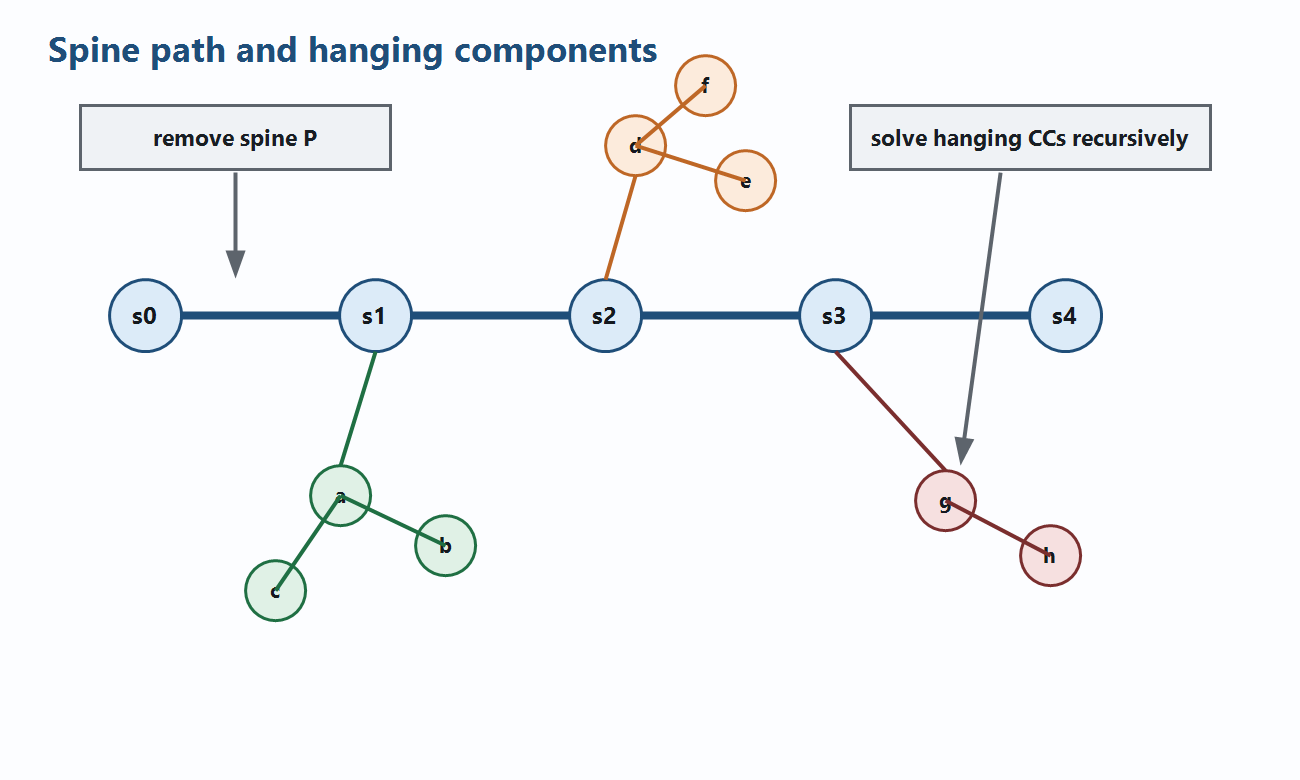
\includegraphics[width=0.92\textwidth]{media/lec26_spine_components.png}
    \caption{A spine path \(P\) and the off-spine connected components that hang from it. Each hanging component becomes an independent recursive subproblem after attachment is fixed.}
    \label{fig:lec26-spine-components}
\end{figure}

\begin{ppdefn}
\ \ppterm{Spine path}\index{spine path} means a root-to-leaf path selected from a spanning tree of the graph.
It acts as the serial backbone of the DFS tree.
The vertices not on the path are partitioned into \emph{hanging components}, which can be processed recursively.
\end{ppdefn}

\paragraph{Intuition: Why the spine enables parallelism.}
The spine path can be viewed as isolating the inherently sequential part of DFS. 
Instead of trying to parallelize the entire traversal, the algorithm identifies a single path that preserves the depth-first ordering constraint. 
Once this path is fixed, all remaining vertices lie in subgraphs that are conditionally independent given their attachment to the spine. 
In other words, the spine acts as a \emph{separator}: it absorbs the global ordering constraints, allowing the hanging components to be explored without interfering with each other. 
This transformation converts one long sequential dependency into many smaller independent subproblems, which can be solved in parallel.

\subsection{High-Level Algorithm}

The lecture's divide-and-conquer outline is:

\begin{enumerate}
    \item Compute a spanning tree \(S\) of the graph in parallel.
    \item Extract a root-to-leaf path \(P\) from \(S\). This path is the spine.
    \item Remove or contract all vertices of \(P\) from the graph.
    \item Find the connected components hanging off \(P\).
    \item Assign each component to an attachment vertex on the spine.
    \item Recursively compute DFS trees of the components in parallel.
    \item Merge the recursive trees into one global DFS tree.
    \item Verify the DFS property if the construction needs an explicit certification step.
\end{enumerate}

\begin{ppkey}
\ The algorithm moves the serial part into a path and tries to make the remaining work independent.
This is the same divide-and-conquer instinct used in many parallel algorithms: isolate a separator, solve the pieces, and merge carefully.
\end{ppkey}

\subsection{Why a Spanning Tree Helps}

A spanning tree gives a connected skeleton of the graph.
From that skeleton we can select a root-to-leaf path.
The path is not arbitrary: it provides a chain along which DFS numbers can be ordered before placing the hanging recursive blocks.

\begin{ppnote}
\ For DFS construction, the spanning tree is a structural tool.
If the graph is weighted and we compute a minimum spanning tree, that tree is certainly a spanning tree.
If the graph is unweighted, the weights may be artificial tie-breakers.
The DFS procedure needs connectivity and a path skeleton, not the optimality of a minimum spanning tree.
\end{ppnote}

\section{Parallel Spanning Tree Construction}
\label{sec:parallel-kruskal}
\index{parallel Kruskal}
\index{Boruvka algorithm}

The slides describe the spanning-tree step using parallel Kruskal-style ideas and Boruvka rounds.
The common goal is to connect components by repeatedly selecting safe edges in parallel.

\subsection{Parallel Sorting of Edges}

Kruskal's algorithm begins by sorting edges by weight.
Sorting is a well-understood parallel primitive.
One simple strategy is:

\begin{enumerate}
    \item Split the edge list into \(p\) chunks.
    \item Sort each chunk locally in parallel.
    \item Merge the sorted chunks using a parallel merge tree.
\end{enumerate}

For example, the edge-weight list
\[
    [38, 27, 43, 3, 9, 82, 10, 19]
\]
may be split across two processors:
\[
    \begin{aligned}
    T_1 &: [38,27,43,3] \to [3,27,38,43],\\
    T_2 &: [9,82,10,19] \to [9,10,19,82].
    \end{aligned}
\]
The two sorted sublists are then merged.

\begin{ppdefn}
\ \ppterm{Parallel merge}\index{parallel merge} merges two sorted arrays by choosing a splitter in one array, binary-searching its position in the other array, and recursively merging the left and right halves in parallel.
The split creates independent subproblems while preserving sorted order.
\end{ppdefn}

\begin{ppprogram}{Recursive parallel merge idea}{prog:parallel-merge}
\begin{lstlisting}[language=C]
parallel_merge(A, B):
    if |A| + |B| is small:
        merge serially
        return

    ensure |A| >= |B|
    x = median element of A
    k = lower_bound(B, x)

    // Elements before A[mid] and before B[k] belong to the left output.
    spawn parallel_merge(A_left,  B_left)
    spawn parallel_merge(A_right, B_right)
    sync
\end{lstlisting}
\end{ppprogram}

The exact complexity depends on the merge implementation and machine model.
The important structural point is that binary search finds a correct split, after which the two halves can proceed independently.
Across many chunks, a tree of merge stages reduces \(p\) sorted lists to one sorted list.

\subsection{Boruvka Rounds}

After sorting, the lecture moves to a Boruvka-style component contraction.
Initially, every vertex is its own component.
In each round:

\begin{enumerate}
    \item Every component finds its minimum-weight outgoing edge.
    \item Selected edges are de-duplicated because two components may choose the same edge.
    \item The chosen edges are added to the forest.
    \item Components connected by chosen edges are contracted into super-vertices.
\end{enumerate}

\begin{ppdefn}
\ \ppterm{Boruvka round}\index{Boruvka round} is a parallel phase in which each current component chooses one cheapest outgoing edge.
All such choices can be made concurrently because each component's local minimum can be computed independently.
\end{ppdefn}

Deduplication matters.
If component \(C_1\) selects edge \((A,C)\) and component \(C_2\) also selects the same edge \((A,C)\), the edge should be inserted only once.
A parallel scan or sort-by-edge-id can compact the selected list into unique edges.

\begin{ppkey}
\ Boruvka rounds are parallel because the algorithm asks many components the same local question at the same time:
``What is your cheapest outgoing edge?''
The contraction step then reduces the number of components, often by a constant factor per round.
\end{ppkey}

\subsection{Parallel Union--Find with Pointer Jumping}
\label{sec:union-find-pointer-jumping}
\index{union--find}
\index{pointer jumping}

Once the algorithm has selected de-duplicated edges such as
\[
    (A,C),\quad (B,E),\quad (B,D),\quad (D,F),
\]
it must update the component structure.
This is the job of union--find.
The parallel version uses parent pointers and pointer jumping to compress paths.

\begin{ppdefn}
\ \ppterm{Pointer jumping}\index{pointer jumping} repeatedly replaces a node's parent by its grandparent:
\[
    parent[v] \gets parent[parent[v]].
\]
After \(O(\log n)\) synchronous rounds on a tree-like parent structure, long paths shrink rapidly toward their roots.
\end{ppdefn}

\begin{ppprogram}{Pointer jumping for component roots}{prog:pointer-jumping}
\begin{lstlisting}[language=C]
parallel_find_roots(parent):
    changed = true
    while changed:
        changed = false
        for each vertex v in parallel:
            old = parent[v]
            parent[v] = parent[parent[v]]
            if parent[v] != old:
                changed = true
\end{lstlisting}
\end{ppprogram}

For an edge \((u,v)\), the edge crosses components exactly when
\[
    Find(u) \neq Find(v).
\]
This gives a constant-time test after the roots have been computed.
Each processor can inspect one edge, record whether it is cross-component, and contribute its weight to a parallel minimum reduction.

\begin{pppitfall}
\ Parallel union--find must be designed carefully.
If many processors update parent pointers without a consistent rule, they can create cycles in the parent forest.
Practical implementations use deterministic linking rules, atomic compare-and-swap, or phased algorithms to keep the structure well formed.
\end{pppitfall}

\section{Extracting a Root-to-Leaf Path}
\label{sec:extract-root-leaf-path}

After computing a spanning tree \(S\), the divide-and-conquer DFS algorithm needs a root-to-leaf path.
The lecture presents an Euler tour approach followed by parallel list ranking.

\subsection{Euler Tour of a Tree}
\index{Euler tour}

Take every undirected tree edge \(\{u,v\}\) and replace it by two directed arcs:
\[
    u \to v
    \qquad\text{and}\qquad
    v \to u.
\]
The Euler tour is represented by a \texttt{next} pointer on each directed arc.
The pointer tells us which arc is visited next in the tree traversal.

\begin{figure}[h]
    \centering
    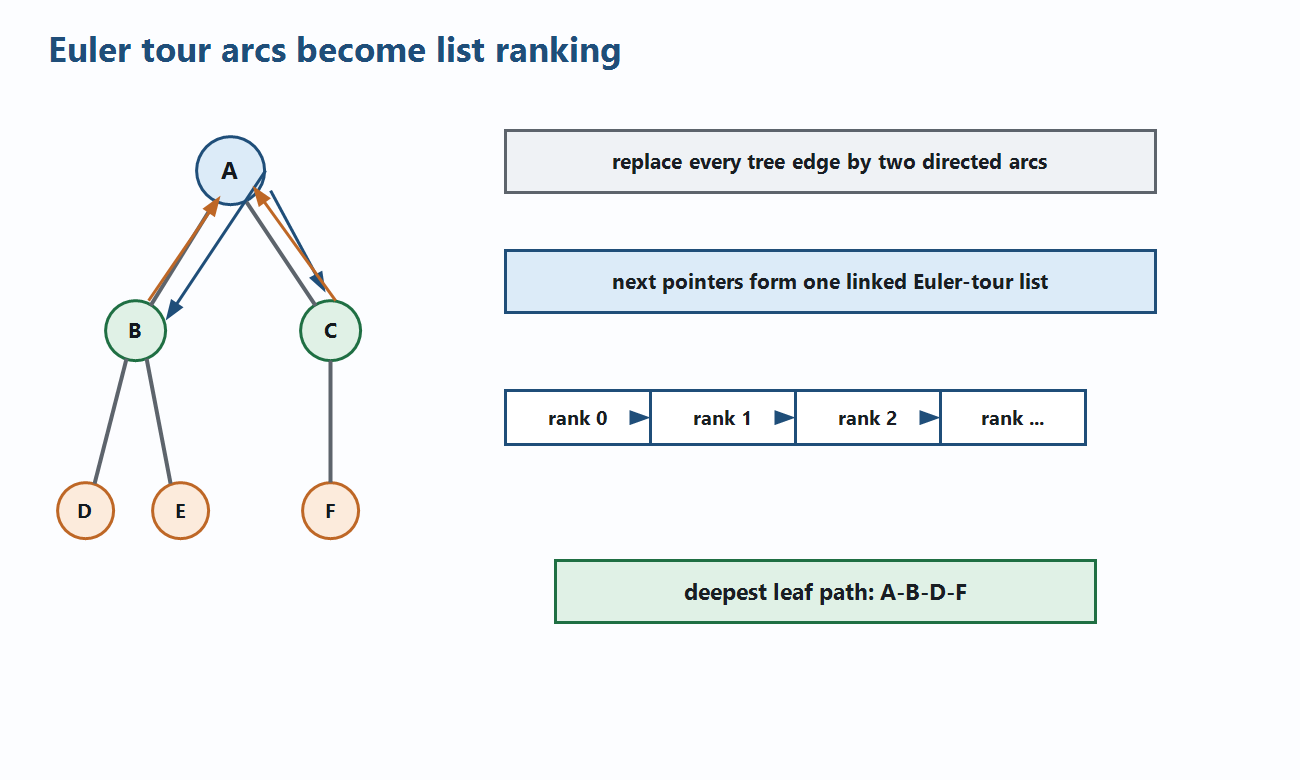
\includegraphics[width=0.92\textwidth]{media/lec26_euler_list_ranking.png}
    \caption{Euler tour construction. Directed tree arcs are linked by next pointers, converting tree traversal into a list-ranking problem.}
    \label{fig:lec26-euler-list-ranking}
\end{figure}

The next-pointer rules are:

\begin{enumerate}
    \item For an entering arc \(u \to v\), if \(v\) has children, the next arc goes from \(v\) to its first child.
    If \(v\) is a leaf, the next arc is \(v \to u\), immediately returning to the parent.
    \item For a returning arc \(v \to u\), the next arc out of \(u\) goes to the next child after \(v\).
    If \(v\) was the last child of \(u\), the next arc returns from \(u\) to \(parent(u)\).
    \item At the root, after the last child has returned, the tour terminates or wraps to a sentinel.
\end{enumerate}

\begin{ppkey}
\ The point of the Euler tour representation is that every arc's successor can be computed locally from parent/child ordering.
Once the successor pointers exist, the tree problem becomes a linked-list problem.
\end{ppkey}

\subsection{Parallel List Ranking}
\index{list ranking}

List ranking assigns to every item in a linked list its distance from the beginning of the list.
With Euler-tour arcs, those ranks encode enough information to recover depths and root-to-leaf paths.

\begin{ppdefn}
\ \ppterm{List ranking}\index{list ranking} computes the rank of every node in a linked list in parallel.
Pointer jumping is again the central trick: each item skips over its successor while accumulating the skipped distance.
\end{ppdefn}

\begin{ppprogram}{List ranking by pointer jumping}{prog:list-ranking}
\begin{lstlisting}[language=C]
parallel_list_rank(next):
    for each list item x in parallel:
        rank[x] = 1

    while next[x] is not NIL for some x:
        for each item x in parallel:
            if next[x] != NIL:
                rank[x] = rank[x] + rank[next[x]]
                next[x] = next[next[x]]
\end{lstlisting}
\end{ppprogram}

Once depths are known, the algorithm can reconstruct paths from leaves to the root in parallel.
The deepest leaf gives a natural root-to-leaf path.
In the example shown in the lecture, the selected path is
\[
    A \to B \to D \to F.
\]
This path becomes the spine for the next divide-and-conquer step.

\section{Finding Hanging Components}
\label{sec:hanging-components}

Let \(P\) be the selected spine path.
Remove the vertices of \(P\) from the graph.
The remaining vertices form one or more connected components.
Each of these components is a hanging subproblem.

\subsection{Off-Spine Parent Initialization}

The lecture describes a parent-pointer method.
For every off-spine vertex \(v\), initialize:
\[
off\_parent[v] =
\begin{cases}
parent[v], & \text{if } parent[v] \text{ is also off-spine},\\
v,         & \text{otherwise}.
\end{cases}
\]
Then repeatedly apply pointer jumping:
\[
    off\_parent[v] \gets off\_parent[off\_parent[v]].
\]
After enough rounds, vertices in the same off-spine tree component point to the same representative.

\begin{ppprogram}{Off-spine component discovery}{prog:off-spine-components}
\begin{lstlisting}[language=C]
find_hanging_components(TreeParent parent, Path P):
    for each vertex v not in P in parallel:
        if parent[v] not in P:
            off_parent[v] = parent[v]
        else:
            off_parent[v] = v

    repeat O(log n) pointer-jumping rounds:
        for each vertex v not in P in parallel:
            off_parent[v] = off_parent[off_parent[v]]
\end{lstlisting}
\end{ppprogram}

\begin{ppnote}
\ If the original graph has non-tree edges among off-spine vertices, the full connected-component computation must account for those edges as well.
The same union--find idea applies: union all off-spine edges whose endpoints are both outside \(P\), then pointer-jump to representatives.
\end{ppnote}

\section{Attaching Components to the Spine}
\label{sec:attach-components}

A hanging component may have edges to multiple vertices on the spine.
To obtain a deterministic DFS-like structure, the lecture uses a simple rule:
attach the component to the deepest spine vertex it touches.

Let the spine be ordered as
\[
    P = (s_0, s_1, \ldots, s_k),
\]
where \(s_0\) is closest to the root and \(s_k\) is deepest.
For a component \(C_i\), inspect all edges \((u,s_j)\) where \(u \in C_i\) and \(s_j \in P\).
Compute
\[
    j^\star = \max \{j : \exists u \in C_i \text{ such that } (u,s_j) \in E\},
    \qquad
    attach(C_i) = s_{j^\star}.
\]

\begin{ppprogram}{Deepest-spine attachment rule}{prog:deepest-attachment}
\begin{lstlisting}[language=C]
attach_components_to_spine(components C, path P):
    for each component C_i in parallel:
        best_index = -1
        best_entry = NIL

        for each edge (u, s_j) with u in C_i and s_j in P:
            if j > best_index:
                best_index = j
                best_entry = u

        attach_vertex[C_i] = s_best_index
        recursive_root[C_i] = best_entry
\end{lstlisting}
\end{ppprogram}

\begin{ppkey}
\ Deepest attachment prevents a component from being pulled upward when it also touches a lower spine vertex.
This is important because DFS ordering should finish deeper opportunities before returning to shallower alternatives.
\end{ppkey}

\subsection{Recursive Calls}

After attachment, each component becomes an independent recursive graph problem.
If \(C_i\) attaches to spine vertex \(s_j\), then one entry vertex inside \(C_i\) is chosen as the recursive root.
The lecture mentions deterministic choices such as:

\begin{itemize}
    \item the first edge in the adjacency-list order,
    \item the smallest endpoint label,
    \item or another fixed tie-breaking rule.
\end{itemize}

The recursive calls can run in parallel because the components are vertex-disjoint.

\begin{pppitfall}
\ The root choice must be deterministic if the algorithm is expected to be reproducible.
Otherwise two executions may produce different valid trees, which is often acceptable for correctness but inconvenient for debugging and testing.
\end{pppitfall}

\section{Merging Recursive DFS Trees}
\label{sec:parallel-tree-merging}
\index{tree merging}

After recursively computing DFS trees for the hanging components, we must merge everything into one global DFS tree.
This is where the algorithm must be careful: a collection of locally valid DFS trees is not automatically a globally valid DFS tree.

\subsection{Merge Invariants}

The lecture states three invariants for the merge:

\begin{enumerate}
    \item \textbf{Attachment edge:} the edge from the spine vertex to the component root becomes a tree edge.
    \item \textbf{Preorder respect:} the spine vertex is numbered before all vertices in its hanging component.
    \item \textbf{Non-tree edge classification:} every non-tree edge is classified using the DFS intervals of its endpoints.
\end{enumerate}

\begin{ppdefn}
\ \ppterm{DFS interval}\index{DFS interval} for a vertex \(u\) is the range
\[
    [dfs[u],\; dfs[u] + size[u] - 1],
\]
where \(dfs[u]\) is the preorder number of \(u\), and \(size[u]\) is the size of \(u\)'s DFS subtree.
A vertex \(v\) is a descendant of \(u\) exactly when \(dfs[v]\) lies inside \(u\)'s interval.
\end{ppdefn}

\subsection{Computing Global DFS Numbers}

Suppose spine vertex \(s_j\) has a hanging component block of size \(block\_size[s_j]\).
The global DFS number of spine vertex \(s_k\) is:
\[
    dfs[s_k] = k + \sum_{j < k} block\_size[s_j],
\]
assuming each earlier spine vertex contributes one slot for itself plus its attached block.
This is exactly the kind of computation prefix sums are meant for.

\paragraph{Intuition: Why prefix sums solve the merge problem.}
The merge step can be understood as assigning each subtree a contiguous segment in the global DFS order. 
Conceptually, we can imagine laying out the spine vertices and their attached component blocks in a linear sequence. 
Each item in this sequence occupies a number of slots equal to its subtree size. 
The key challenge is to determine where each item starts in this global ordering without processing them one by one. 
Prefix sums solve exactly this problem: by computing the cumulative sizes of all preceding items, each subtree can independently determine its starting index. 
This allows all DFS numbers to be assigned in parallel while still preserving the correct depth-first ordering structure.

\begin{figure}[h]
    \centering
    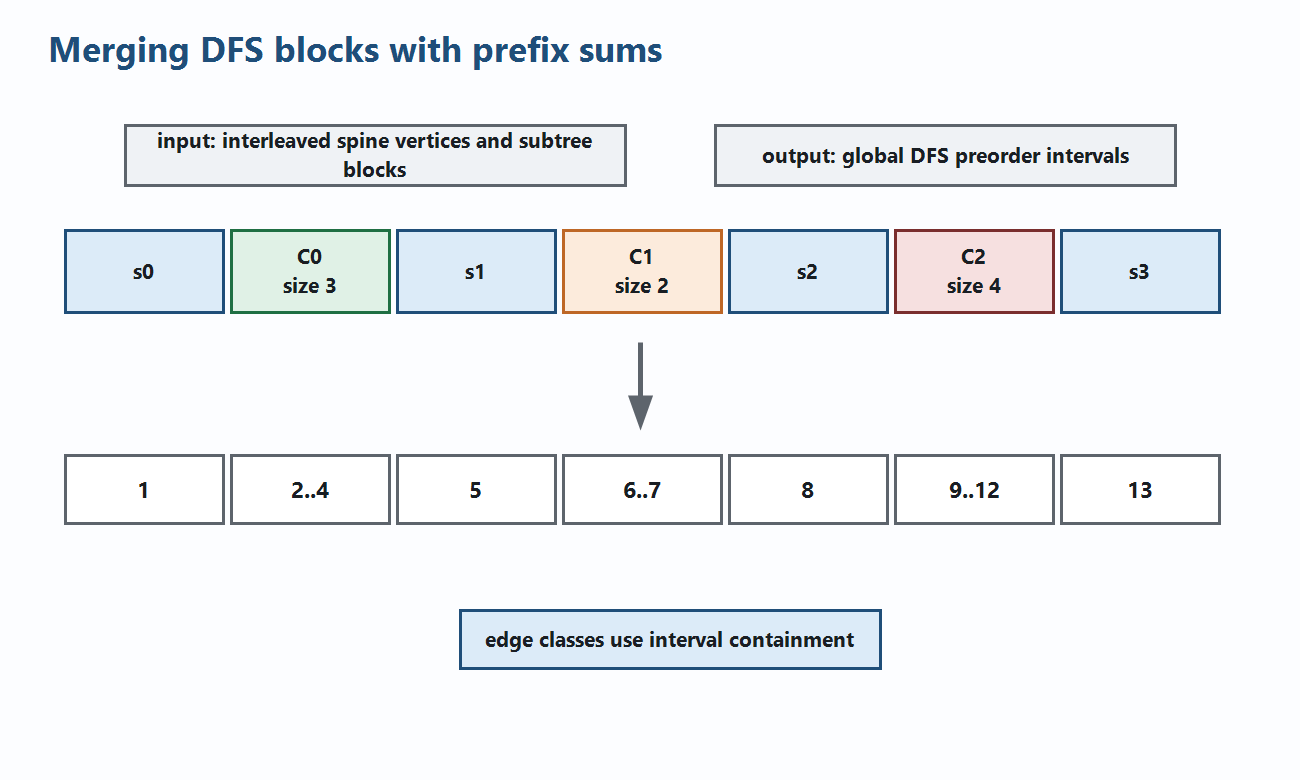
\includegraphics[width=0.92\textwidth]{media/lec26_prefix_merge.png}
    \caption{Merging by prefix sums. Spine vertices and component blocks form an interleaved array; prefix sums assign each block its global DFS interval.}
    \label{fig:lec26-prefix-merge}
\end{figure}

\begin{ppprogram}{Prefix-sum merge numbering}{prog:prefix-merge-numbering}
\begin{lstlisting}[language=C]
merge_numbering(path P, attached_blocks B):
    // Interleave spine vertices and their component blocks.
    A = []
    for j = 0 to |P|-1:
        append A, item(type = SPINE, size = 1, vertex = P[j])
        if B[j] exists:
            append A, item(type = BLOCK, size = |B[j]|, component = B[j])

    start = parallel_prefix_sum(A.size)

    for each item A[t] in parallel:
        if A[t].type == SPINE:
            dfs[A[t].vertex] = start[t]
        else:
            offset all local DFS numbers in A[t].component by start[t]
\end{lstlisting}
\end{ppprogram}

\begin{ppkey}
\ The prefix sum is the merge glue.
It assigns disjoint global number ranges to subtrees without serially walking every component in spine order.
\end{ppkey}

\subsection{Classifying Non-Tree Edges}

After global DFS numbers and subtree sizes are known, a non-tree edge \((u,v)\) can be classified by interval containment:

\begin{itemize}
    \item If \(dfs[u] < dfs[v]\) and
    \[
        dfs[v] \le dfs[u] + size[u] - 1,
    \]
    then \(v\) lies in \(u\)'s subtree. The edge is a forward edge from ancestor to descendant.
    \item If \(dfs[v] < dfs[u]\) and
    \[
        dfs[u] \le dfs[v] + size[v] - 1,
    \]
    then \(u\) lies in \(v\)'s subtree. The edge is a back edge from descendant to ancestor.
    \item Otherwise the edge is a cross edge.
\end{itemize}

For undirected DFS, cross edges are a warning sign: a valid DFS tree of an undirected graph should not have cross edges between unrelated subtrees.
Therefore classification can also serve as a verification step.

\begin{pppitfall}
\ Forward, back, and cross edge terminology is standard for directed DFS.
For undirected graphs, every non-tree edge in a correct DFS tree should connect an ancestor and a descendant.
So in the undirected setting, a cross edge usually indicates that the proposed merge is not a valid DFS tree.
\end{pppitfall}

\section{Putting the Pieces Together}
\label{sec:lec26-putting-together}

The full algorithm is best understood as a pipeline of parallel primitives:

\begin{enumerate}
    \item Parallel sort/selection builds a spanning tree skeleton.
    \item Euler tour plus list ranking extracts a deep root-to-leaf path.
    \item Pointer jumping and union--find identify off-spine components.
    \item A deepest-attachment rule assigns each component to a spine vertex.
    \item Recursive calls solve independent components.
    \item Prefix sums merge local DFS number ranges into a global order.
    \item Interval tests verify or classify non-tree edges.
\end{enumerate}

\begin{ppprogram}{Divide-and-conquer parallel DFS skeleton}{prog:dc-parallel-dfs}
\begin{lstlisting}[language=C]
parallel_DFS(Graph G, Vertex r):
    if G is small:
        return serial_DFS(G, r)

    S = parallel_spanning_tree(G)
    P = deepest_root_to_leaf_path(S, r)

    components = connected_components(G without vertices of P)
    attachments = deepest_spine_attachment(components, P)

    for each component C_i in parallel:
        T_i = parallel_DFS(C_i, root_i)

    T = merge_spine_and_recursive_trees(P, T_i, attachments)
    verify_or_classify_non_tree_edges(G, T)
    return T
\end{lstlisting}
\end{ppprogram}

\begin{ppkey}
\ This algorithm is not one trick.
It is a composition of standard parallel primitives: sorting, reduction, scan, pointer jumping, list ranking, connected components, recursion, and verification.
That is why parallel graph algorithms often look more elaborate than their serial counterparts.
\end{ppkey}

\subsection{Where Parallelism Appears}

\begin{itemize}
    \item Edge sorting and merging use parallel divide-and-conquer.
    \item Component minimum-edge selection uses parallel reductions.
    \item Deduplication uses sorting, hashing, or scan-style compaction.
    \item Union--find uses parallel pointer updates with path compression.
    \item Euler-tour next pointers are computed independently for arcs.
    \item List ranking uses pointer jumping.
    \item Hanging components are solved recursively in parallel.
    \item Merge numbering uses prefix sums.
\end{itemize}

\subsection{Where Sequential Dependence Remains}

DFS remains difficult because the spine is still a chain.
The algorithm tries to make the chain small enough, or the hanging work large enough, that parallelism is still available.
In worst-case graphs that are essentially paths, DFS has little useful parallelism because the graph itself exposes a long dependence chain.

\begin{ppnote}
\ A good mental model: parallel DFS does not remove the depth-first dependency.
It isolates that dependency into a spine and then parallelizes the subproblems hanging from the spine.
\end{ppnote}

\subsection{Complexity View}

Let \(m = |E|\), \(n = |V|\), and \(p\) be the number of processors.
The exact bounds depend on the implementation choices, but the main costs are:

\begin{itemize}
    \item sorting or selecting edges for the spanning-tree stage,
    \item \(O(\log n)\)-style pointer-jumping phases for components/list ranking under idealized parallel models,
    \item recursive work over disjoint hanging components,
    \item prefix-sum work for merge numbering,
    \item edge-parallel interval tests for verification.
\end{itemize}

The work should remain near-linear or sorting-dominated for a practical implementation.
The span depends heavily on how balanced the spine decomposition is.

\begin{pppitfall}
\ Do not judge a parallel graph algorithm only by the number of processors it uses in one step.
The critical question is whether the algorithm repeatedly creates balanced independent work, or whether it keeps producing one large serial subproblem.
\end{pppitfall}

\subsection{Key Takeaways}

\begin{itemize}
    \item Strict DFS is hard to parallelize because depth-first order creates a long dependency chain.
    \item A work-pool traversal can find reachable vertices in parallel, but it does not guarantee a valid DFS tree.
    \item The divide-and-conquer strategy chooses a spine path, removes it, and recursively solves hanging components.
    \item Parallel spanning-tree construction uses sorting, Boruvka-style edge selection, deduplication, and union--find.
    \item Pointer jumping is a unifying primitive for parent compression, connected components, and list ranking.
    \item Euler tours convert tree traversal into a linked-list ranking problem.
    \item Deepest-spine attachment gives a deterministic rule for placing hanging components.
    \item Prefix sums assign global DFS number ranges during merge.
    \item DFS interval containment classifies non-tree edges and helps verify correctness.
\end{itemize}

\subsection{Exercises}

\begin{ppexercises}
  \ppexercise{Why does exploring all neighbours of a vertex in parallel fail to reproduce serial DFS?}

  \textbf{Answer:} Serial DFS must finish the complete recursive subtree of one neighbour before moving to the next neighbour. If two neighbours are explored simultaneously, their discoveries interleave, so the parent tree may not satisfy the DFS ancestor--descendant property.

  \ppexercise{In Program~\ref{prog:work-pool-search}, why is an atomic compare-and-swap needed for \texttt{visited[v]}?}

  \textbf{Answer:} Two processors may discover the same vertex at the same time. The atomic operation ensures that exactly one processor changes \texttt{visited[v]} from false to true and therefore exactly one processor assigns \texttt{parent[v]}.

  \ppexercise{Explain how pointer jumping reduces the height of a parent-pointer tree.}

  \textbf{Answer:} Each round replaces a vertex's parent by its grandparent. A path of length \(L\) is roughly halved each round, so after \(O(\log L)\) rounds, vertices point close to or directly at the root.

  \ppexercise{Let a spine be \(s_0,s_1,s_2\), and suppose the attached component block sizes are \(2,0,3\). What global DFS numbers are assigned to the spine vertices if numbering starts at \(1\)?}

  \textbf{Answer:} The order is \(s_0\), block of size \(2\), \(s_1\), \(s_2\), block of size \(3\). Thus \(dfs[s_0]=1\), \(dfs[s_1]=4\), and \(dfs[s_2]=5\).

  \ppexercise{Given \(dfs[u]=4\), \(size[u]=6\), \(dfs[v]=8\), and \(size[v]=2\), classify edge \((u,v)\).}

  \textbf{Answer:} The interval of \(u\) is \([4,9]\), and \(dfs[v]=8\) lies inside it. Thus \(v\) is a descendant of \(u\), so the edge is ancestor-to-descendant from \(u\)'s perspective.
\end{ppexercises}

\section*{References}
\addcontentsline{toc}{section}{References}

This chapter is based on Lecture~26, \emph{Parallel Algorithms}, from \texttt{lec26-PA.pdf}.
For background on parallel graph algorithms, spanning trees, prefix sums, and parallel performance models, see standard parallel-programming references such as Pacheco's \emph{An Introduction to Parallel Programming}.

\section*{Contributions}
\addcontentsline{toc}{section}{Contributions}

This chapter transcription and expansion was prepared from the Lecture~26 slide deck.
The diagrams in Figures~\ref{fig:lec26-work-pool}, \ref{fig:lec26-spine-components}, \ref{fig:lec26-euler-list-ranking}, and \ref{fig:lec26-prefix-merge} were redrawn as manuscript figures to illustrate the algorithms without relying on raw slide screenshots.

\subsection*{Namit Jain (2023CS10483)}
Lecture~26 transcription, chapter structuring, explanations, pseudocode, exercises, and manuscript figures.

\subsection*{Additional Contributors}
Names and contributions to be added.
